\documentclass[border=10pt]{standalone}
\usepackage{pgfplots}
\pgfplotsset{compat=1.18, trig format plots=rad}
\begin{document}
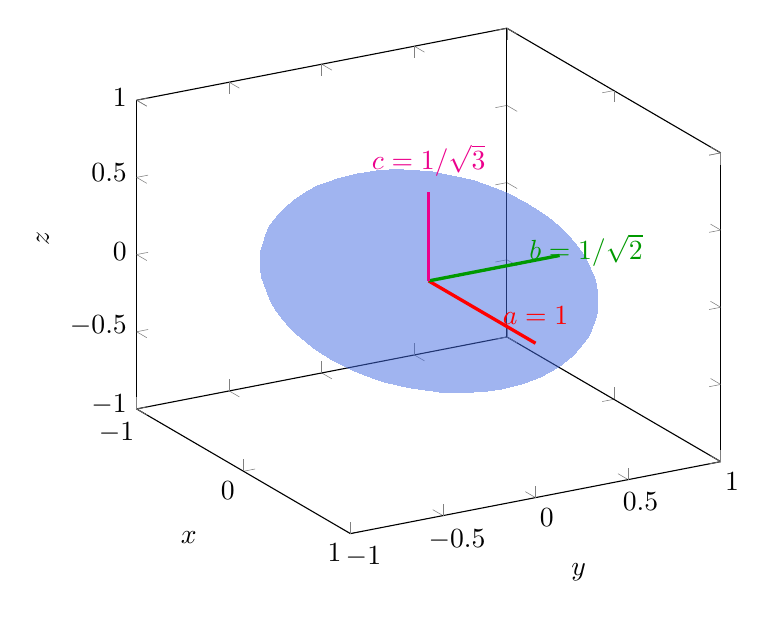
\begin{tikzpicture}
\begin{axis}[
  view={60}{25},
  xlabel=$x$, ylabel=$y$, zlabel=$z$,
  xmin=-1, xmax=1, ymin=-1, ymax=1, zmin=-1, zmax=1,
  samples=45, samples y=35,
  width=9cm, height=8cm,
]
\addplot3[surf, domain=0:2*pi, domain y=0:pi, shader=interp,
          colormap={royal}{rgb255(0cm)=(65,105,225); rgb255(1cm)=(65,105,225)},
          opacity=0.5]
  ({sin(y)*cos(x)}, {sin(y)*sin(x)/sqrt(2)}, {cos(y)/sqrt(3)});
\addplot3[red, very thick] coordinates {(0,0,0) (1,0,0)};
\addplot3[green!60!black, very thick] coordinates {(0,0,0) (0,0.7071,0)};
\addplot3[magenta, very thick] coordinates {(0,0,0) (0,0,0.5774)};
\node[red] at (axis cs:1.0,0,0.18) {$a=1$};
\node[green!60!black] at (axis cs:0,0.85,0) {$b=1/\sqrt{2}$};
\node[magenta] at (axis cs:0,0,0.78) {$c=1/\sqrt{3}$};
\end{axis}
\end{tikzpicture}
\end{document}
